% 근거: chapter4-prep-v1/A2/hop-f1-figure-data.jsonl,
%       chapter4-prep-v1/A3/win-tie-loss.json, analysis.json
% 그림 삽입에는 graphicx가 필요하다. 저장소 루트에서 컴파일한다.
\subsection{질문 조건에 따른 성능 차이}
\label{sec:ch4_subgroups}

전체 평균에서 관찰된 차이가 질문 조건에 따라 어떻게 달라지는지
공식 hop별로 살펴보았다. 그림~\ref{fig:ch4_hop_f1}과 같이,
1-hop 57문항에서는 Jev의 F1이 76.90점으로 수정 CE의 78.07점보다
1.17점 낮았다. 반면 2-hop 127문항에서는 53.33점에서 57.24점으로
3.91점, 3-hop 42문항에서는 47.91점에서 54.83점으로 6.92점 높았다.
이는 2ㆍ3-hop에서 개선 폭이 큰 점추정 패턴이지만, 층 간 효과 차이의
상호작용을 검정한 결과는 아니다. 공식 hop은 평가 자료의 구분이며
개별 문항의 실제 gold 개수와도 구별한다.

\begin{figure}[htbp]
    \centering
    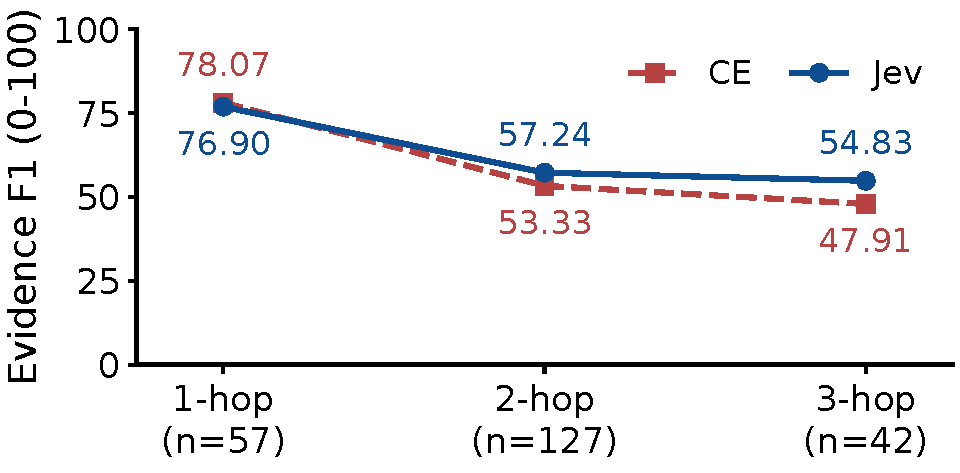
\includegraphics[width=\linewidth]{research/chapter4/figures/hop_f1.pdf}
    \caption{공식 hop별 최종 근거 F1. 표본 수는 각각 57, 127, 42문항이다.
    점은 기술통계이며 층별 신뢰구간은 산출하지 않았다.}
    \label{fig:ch4_hop_f1}
\end{figure}

특히 3-hop에서 모든 gold를 포함한 문항은 두 조건 모두
1개(1/42, 2.38\%)였다. 평균 F1의 증가는 일부 정답 근거의 추가 회수와
양립하지만, 여러 근거를 동시에 갖추는 문제는 여전히 남아 있다.
앞 절의 매핑 상태별 진단에서도 두 집단의 점추정은 Jev가 높았으나,
이러한 하위집단 결과를 모든 질문 조건에 대한 일관된 우월성으로
확장하기는 어렵다.

문항별 대응 비교에서도 개선과 악화가 함께 관찰되었다.
반올림 전 F1 차이에 $10^{-12}$의 동률 허용오차를 적용하면,
Jev가 높은 문항은 32개, 같은 문항은 177개, 수정 CE가 높은 문항은
17개였다. 이 집계는 평균 차이가 일부 문항의 변화에서 발생했음을
보여준다. 문항 간 sourceㆍgold 의존성이 있으므로 해당 개수를
독립 시행의 성공률로 해석하지 않았다.
